\begin{titlepage}
    \centering
    \vspace*{0.5cm}
    
    {\scshape\LARGE ITALOccult Project \par}
    \vspace{0.5cm}
    
    \rule{\linewidth}{0.5mm} \\[0.3cm]
    {\Huge\bfseries Scientific Reference Manual \par}
    \vspace{0.3cm} 
    \rule{\linewidth}{0.5mm} \\[0.8cm]
    
    {\Large\textit{High-Fidelity C++ Library for Asteroid Dynamics\\and Occultation Prediction} \par}
    
    \vspace{1.5cm}
    
    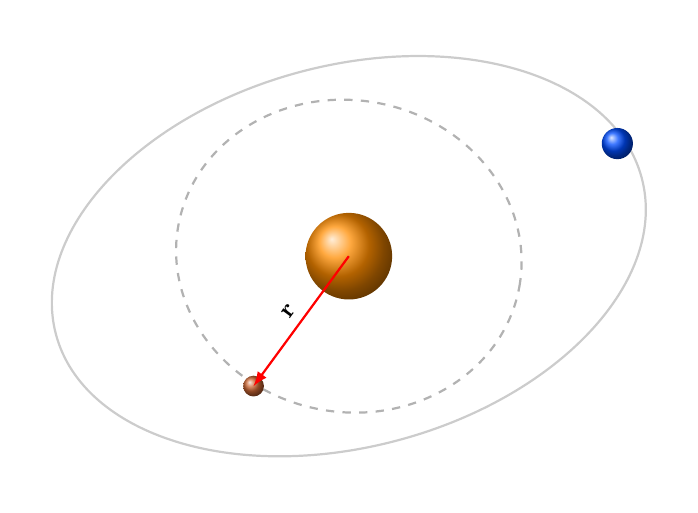
\begin{tikzpicture}[scale=1.1]
        % Abstract representation of solar system dynamics
        % Sun
        \shade[ball color=orange!90!yellow] (0,0) circle (0.5);
        
        % Orbits
        \draw[gray!40, thick, rotate=15] (0,0) ellipse (3.5 and 2.2);
        \draw[gray!60, thick, dashed, rotate=-10] (0,0) ellipse (2.0 and 1.8);
        
        % Bodies
        \shade[ball color=blue!70!cyan] (3.1, 1.3) circle (0.18); % Earth-like
        \shade[ball color=brown!80!red] (-1.1, -1.5) circle (0.12); % Asteroid
        
        % Vector annotation (symbolic)
        \draw[->, >=latex, red, thick] (0,0) -- node[above, sloped, black] {\small $\mathbf{r}$} (-1.1, -1.5);
    \end{tikzpicture}
    
    \vspace{3cm}
    
    {\Large \textbf{Michele Bigi} \par}
    
    \vfill
    
    % --- Controcopertina (Verso Page) ---
    \newpage
    \thispagestyle{empty}
    \null
    \vfill
    
    \begin{flushleft}
        \small
        \textbf{Document Information:}\\
        Version: 1.0.0 \\
        Date: \today \\[0.5cm]
        
        \textit{Validated against JPL DE441 Ephemerides}\\[2cm]
        
        \copyright\ \the\year\ Michele Bigi -- ITALOccult Project\\
        All rights reserved.
    \end{flushleft}

\end{titlepage}
\clearpage
